\documentclass{article}

\usepackage[spanish, mexico]{babel}
\usepackage[utf8]{inputenc}
\usepackage{csvsimple}
\usepackage{listingsutf8}
\usepackage{longtable}
\usepackage{subcaption}
\usepackage{graphicx}
\usepackage{float}

\graphicspath{{figuras/}}

\newcommand{\tab}{\indent\indent}
%\renewcommand{\theenumi}{\alph{enumi})}

\begin{document}
\begin{titlepage}
\centering
\vfill
\rule{\textwidth}{1.6pt}\vspace{-\baselineskip}\vspace{0.1pt}
\rule{\textwidth}{0.4pt}
{\LARGE Universidad Autónoma de Baja California\\
Facultad de Ciencias\\
\textbf{Carrera:} Física\\
\rule{\textwidth}{0.4pt}\vspace{-\baselineskip}\vspace{10pt}
\rule{\textwidth}{1.6pt}
\textbf{Alumnos/Matrículas:} Diego Osvaldo Ochoa de la Cruz 346427\\
Federico Soto Badilla 347428\\
\textbf{Materia:} Instrumentación\\
\textbf{Docente:} Eloisa del Carmen García Canseco\\
\textbf{Proyecto Final}\\
Osciloscopio con Arduino\\
30 de Mayo del 2018\\}
\vfill

\begin{figure}[h]
\begin{subfigure}{0.5\textwidth}
\centering

\includegraphics[scale=0.1]{uabc.png}
\end{subfigure}
\begin{subfigure}{0.5\textwidth}
\centering

\includegraphics[scale=0.1]{fcs.jpg}
\end{subfigure}
\end{figure}
\end{titlepage}

\setcounter{figure}{0}
{\LARGE\textbf{Objetivos}}
\begin{itemize}
\item Aprender a utilizar la tarjeta Arduino
\item Aprender a graficar en tiempo real en Pyhton
\item Utilizar lo aprendido en clase para poder elaborar un osciloscopio
\end{itemize}
 \section{Introducción}
En electrónica, a la hora de querer implementar circuitos electrónicos, es de suma
importancia el conocer el potencial de la onda que se le suministra al circuito, ya que
tener bien conocido ese dato, entre otros, garantiza un buen funcionamiento del circuito
utilizado así como la integridad  del mismo. Para conocerlo es necesario un instrumento
que tenga la capacidad de medir el potencial y así poder tener idea de él.\\
Este instrumento es conocido como osciloscopio y su función es medir y desplegar en
pantalla la forma de la onda así como la amplitud (Voltaje) que tiene la onda que se le
suministra, entre otros datos sobre ella.\\
Un inconveniente de este instrumento es el precio que tiene, el cual es demasiado elevado
para el público en general por lo que tener una alternativa más económica es realmente
útil. Es aquí donde Arduino puede ser útil para poder obtener uno por un precio mucho
menor; sin embargo la exactitud es menor a la que se obtiene con uno comprado ya hecho
pero no deja de ser una opción viable cuando se necesita uno de esos instrumentos.\\
 Este proyecto consiste en implementar, con Arduino, un osciloscopio de bajo costo para
 tener una opción adicional a un osciloscopio ya hecho.\\
Cabe decir que este proyecto es la adaptación de un proyecto ya existente encontrado en
internet.\\

\noindent
\textbf{Lista de Materiales}\\
\textbf{Electrónicos}
\begin{itemize}
\item Arduino UNO
\item Computadora
\item 8 Resistencias de 1kOhm
\end{itemize}
\textbf{Mecánico}
\begin{itemize}
\item Protoboard
\item Jumpers
\end{itemize}
\textbf{Software}
\begin{itemize}
\item Editor de Arduino
\item Python
\end{itemize}

\section{Funcionamiento}
\noindent
\textbf{\underline{Tarjeta Arduino:}} Es una placa para programar basada en un micro controlador
ATMEL, el cual tiene como función recibir instrucciones, guardarlas y ejecutarlas.
Físicamente este dispositivo está compuesto por millones de transistores y otros
componentes que realizan operaciones lógicas y permiten que el micro controlador funcione.
Estas instrucciones que se le dan se escriben utilizando el editor que proporciona
Arduino.\\
Este micro controlador posee entradas y salidas tanto analógicas como digitales. Arduino
se comunica con la computadora a través del puerto serial.\\
El funcionamiento específico del micro controlador dependerá del proyecto que se esté
realizando.\\
\textbf{\underline{Resistencia:}} Es un componente pasivo de dos terminales que se utiliza para
agregar resistencia eléctrica a un circuito. Son usados para reducir el flujo de
corriente, ajustar niveles de señales, dividir voltajes, entre otras aplicaciones.\\
\textbf{\underline{Python:}} Pyhton es un lenguaje de programación interpretado con muchas
librerías orientadas al computo científico entre ellas existen tres que fueron de gran
ayuda en este proyecto:
\begin{itemize}
\item \textbf{matplotlib.pyplot} Que nos permite utilizar funciones para graficar un
conjunto de datos.
\item \textbf{serial} Que nos proporciona una forma de interactuar con el puerto serial de
la computadora para comunicarnos con la tarjeta Arduino.
\item \textbf{drawnow} Proporciona la función del mismo nombre que permite tomar una
gráfica ya hecha y actualizar los datos en ella, esta basada en una librería con el mismo
nombre encontrada en matlab.
\end{itemize}
Cabe mencionar que matlab, entre otros lenguajes, tiene librerías y funciones similares
pero escogimos python porque además de la utilidad que tiene ya estábamos familiarizados
con el lenguaje.\\
\textbf{\underline{Qucs(Quite Universal Circuit Simulator):}} Es un programa hecho para
simulación de circuitos que sigue siendo desarrollado, lo escogimos a inicio del semestre
para utilizarlo en las practicas ya que era la mejor opción que encontramos en Linux
(nuestro sistema operativo al momento), pero existe en otras plataformas y tiene lo
necesario para este proyecto.\\
\begin{figure}[h]
\centering
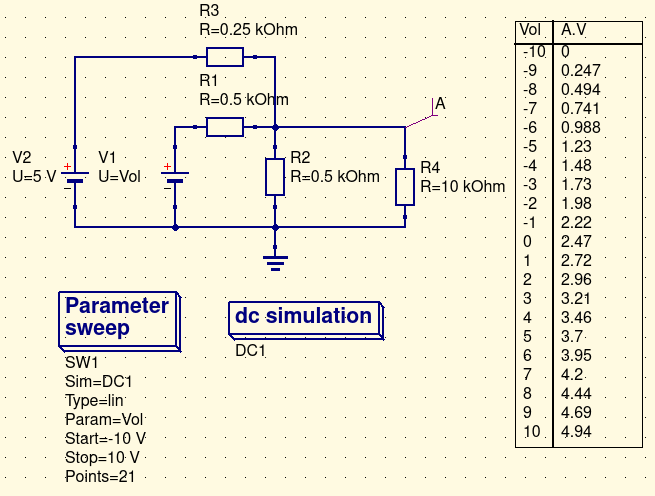
\includegraphics[scale=0.3]{CirSim.png}
\caption{Simulación del circuito en Qucs}
\label{Fig:Cir}
\end{figure}
\begin{figure}[h]
\begin{subfigure}{0.5\textwidth}
\centering
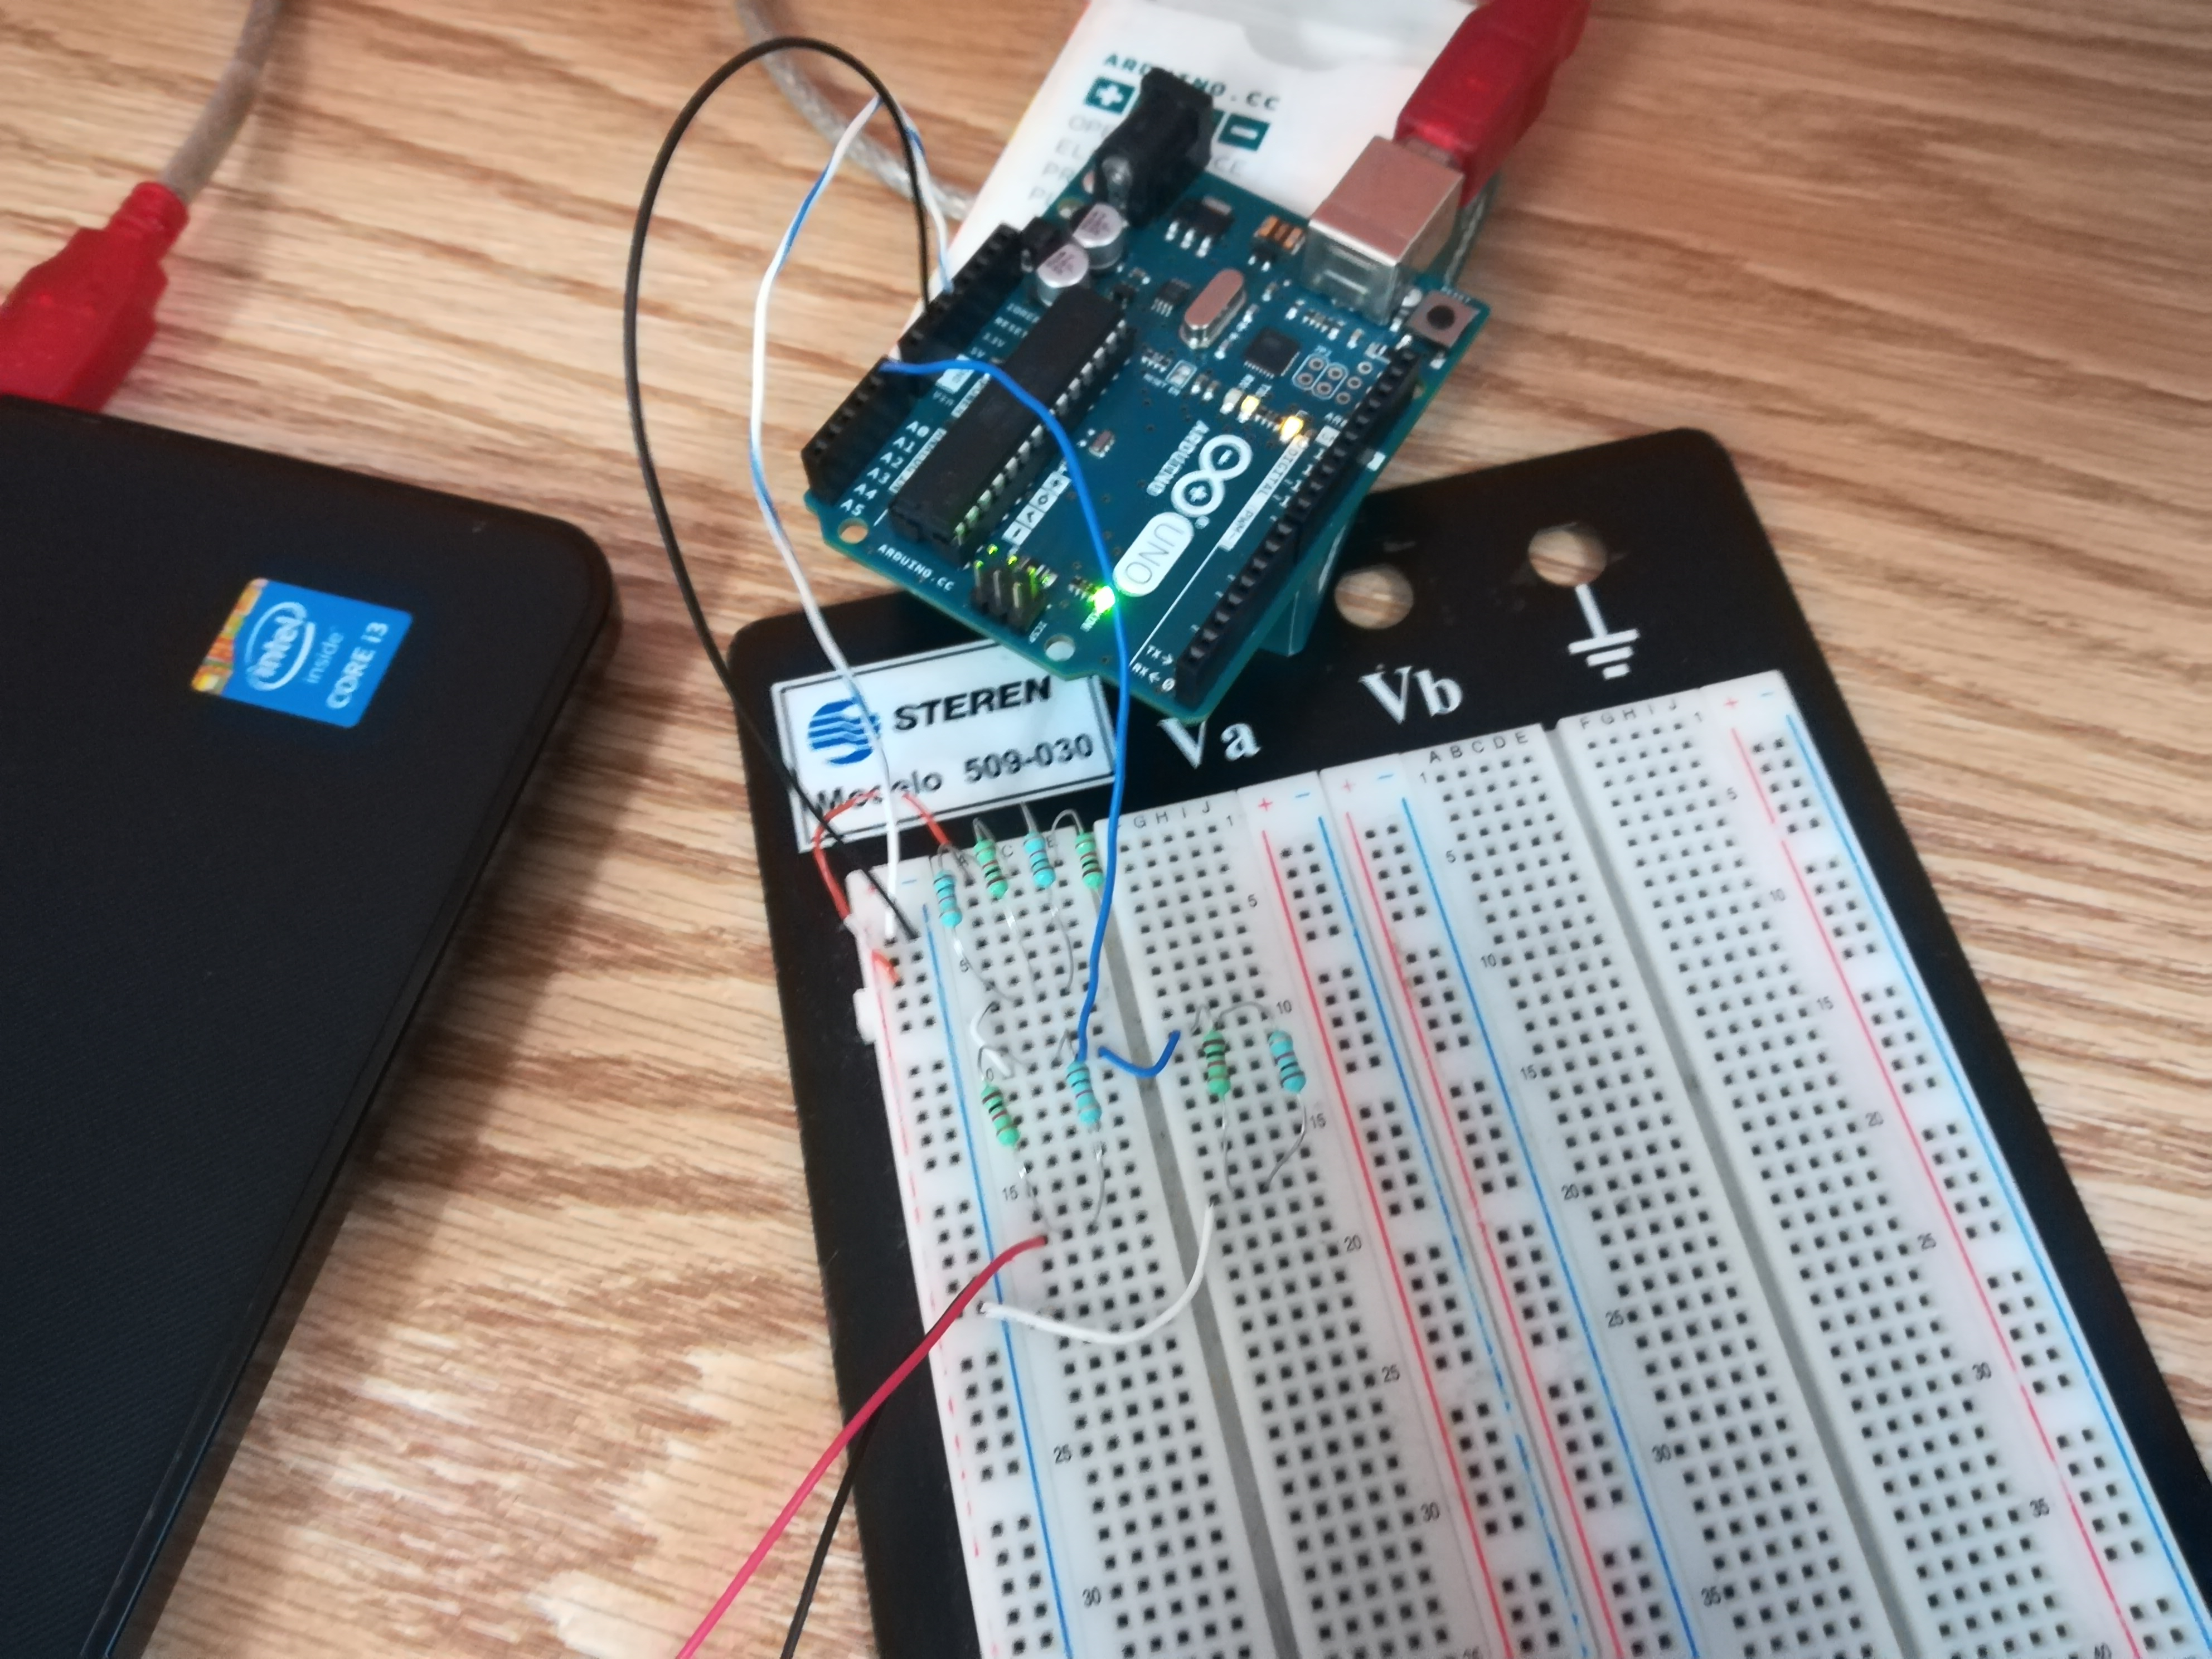
\includegraphics[scale=0.04]{Cir1.jpg}
\end{subfigure}
\begin{subfigure}{0.5\textwidth}
\centering
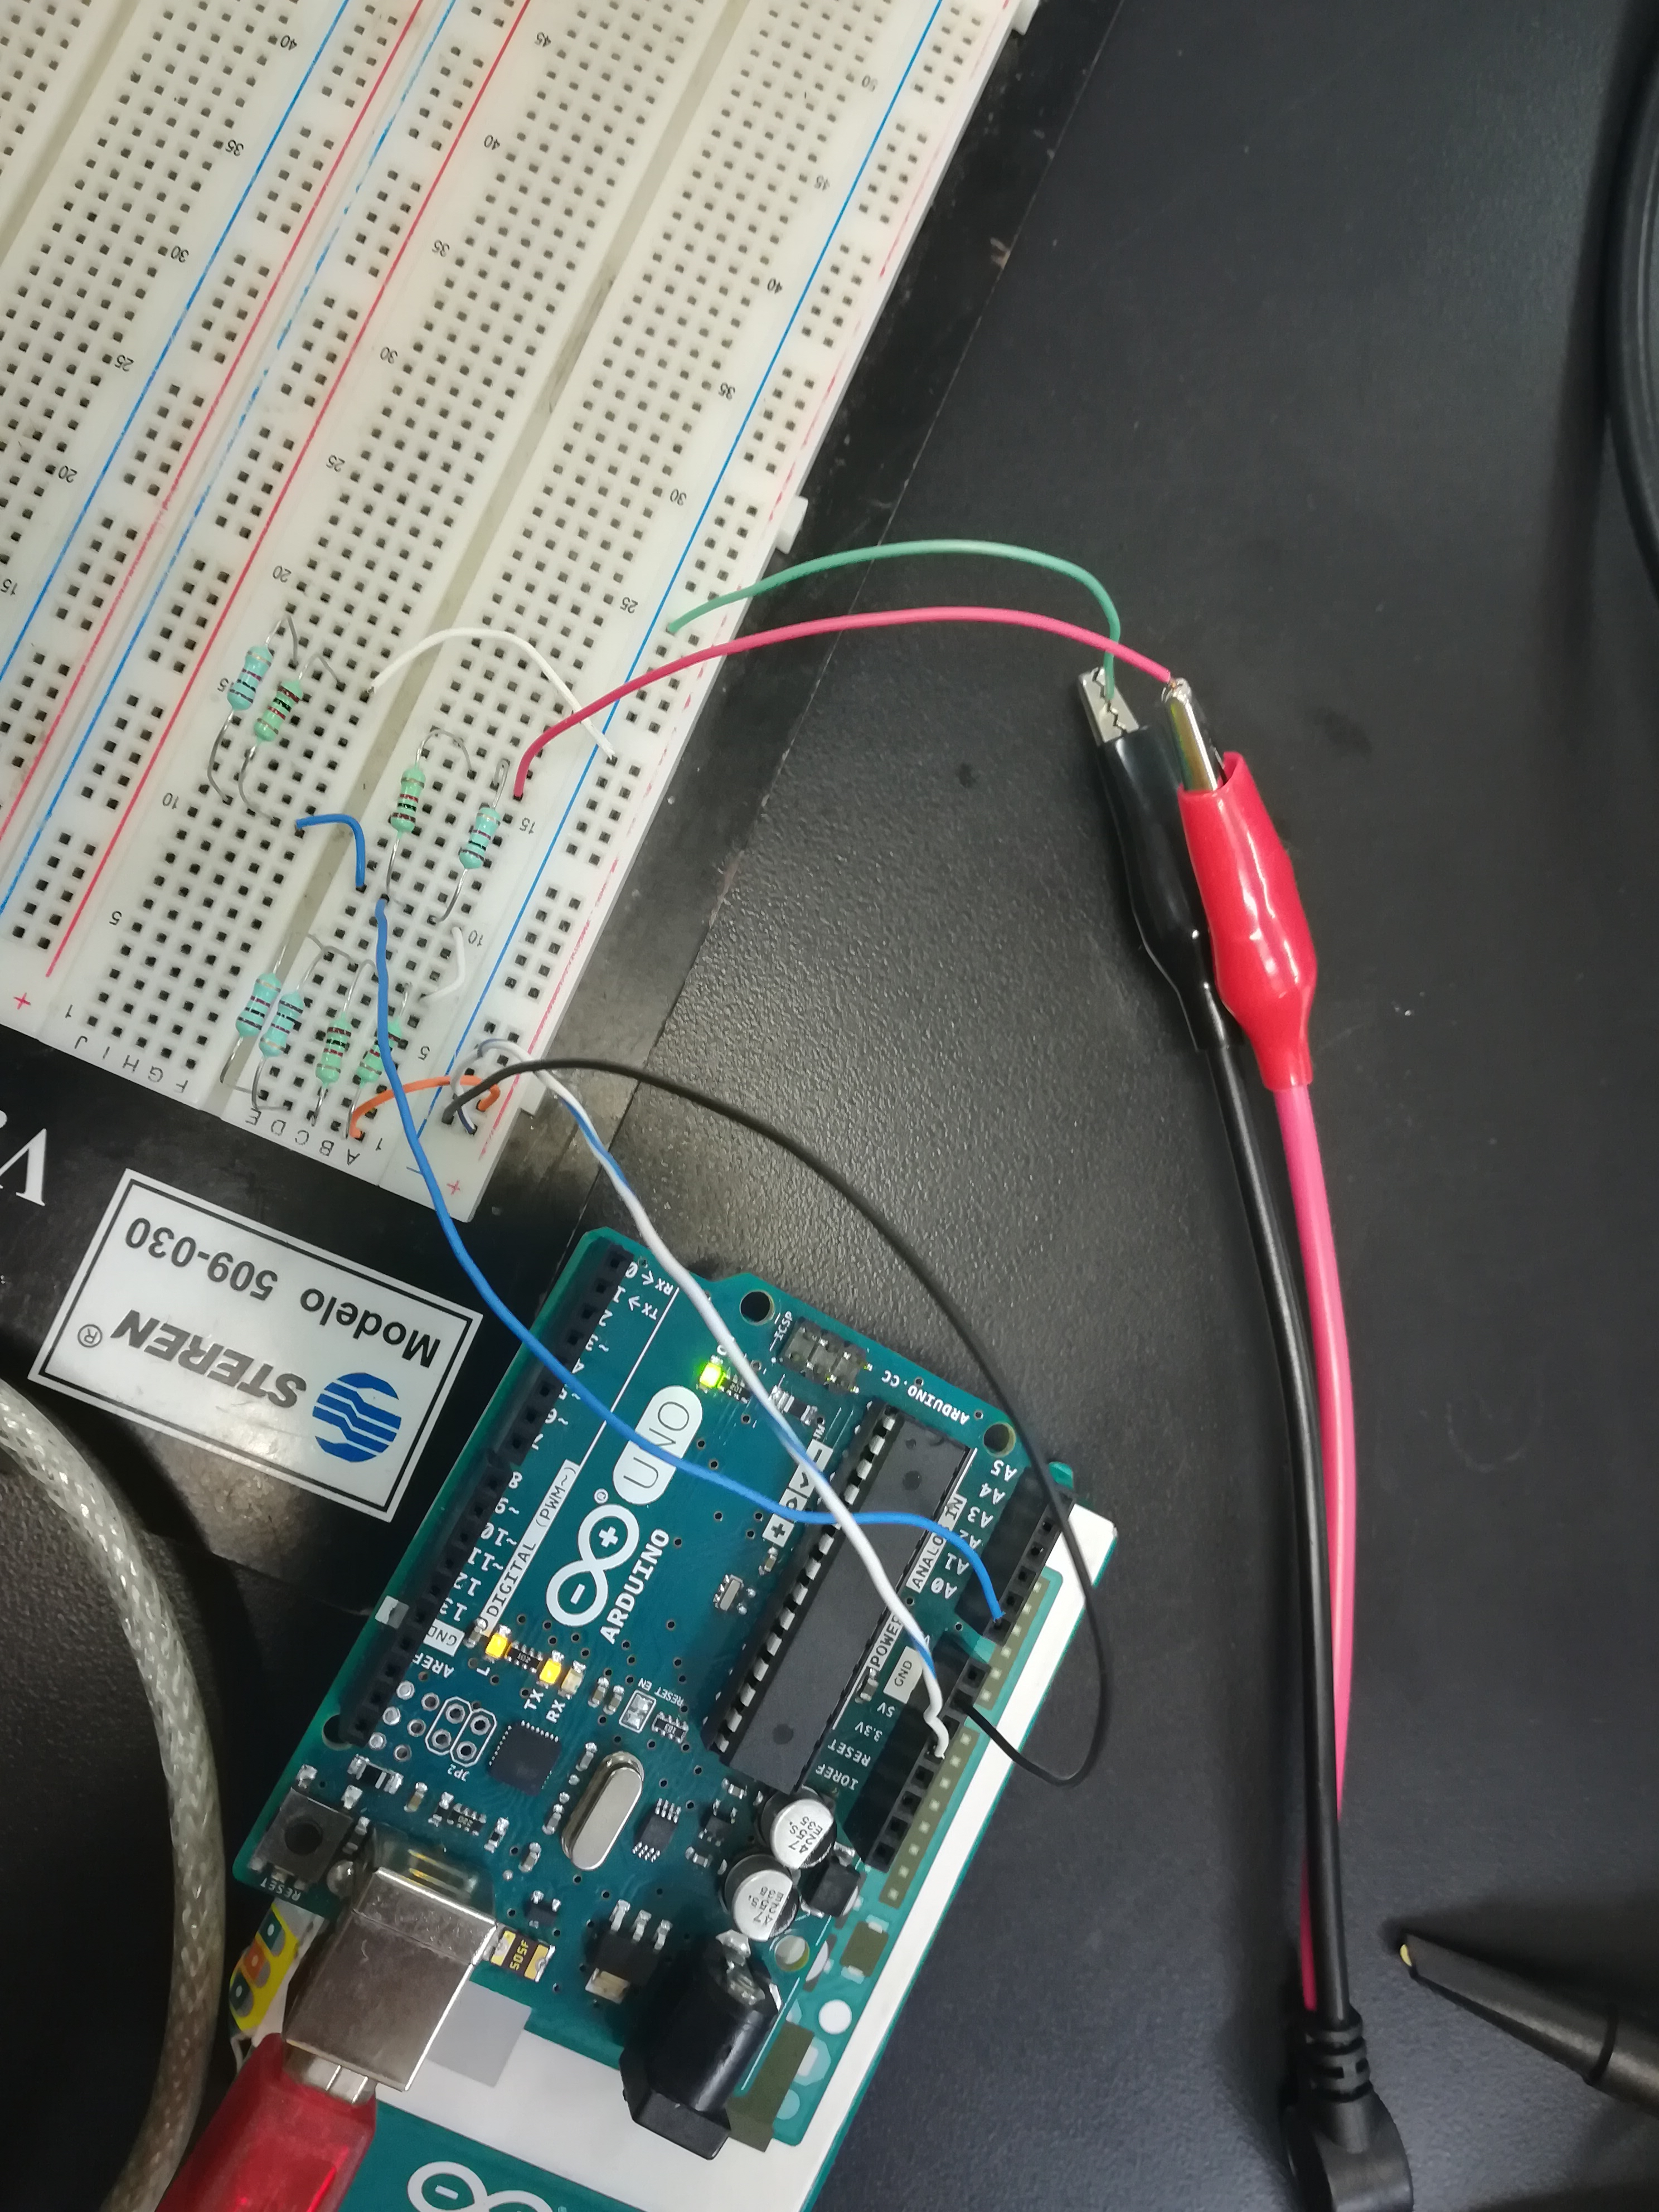
\includegraphics[scale=0.04]{Cir2.jpg}
\end{subfigure}
\caption{Circuito de resistencias conectado al Arduino}
\end{figure}
\lstdefinestyle{Arduino}{
	keywords={void},
	morecomment=[l]{//},
	morecomment=[s]{/*}{*/}}
\lstset{
	inputencoding=utf8/latin1,
	breaklines=true}
\subsection{Código de Arduino}\label{Cod:Ard}
\lstinputlisting[style=Arduino]{../codigo/ReadAnalogVoltage/ReadAnalogVoltage.ino}
\subsection{Código de Python}\label{Cod:Py}
\lstinputlisting[language=Python]{../codigo/osciloscopio.py}

\section{Desarrollo del proyecto}
\begin{enumerate}
\item Ahora procedemos a elaborar el circuito que permitirá que el Arduino lea voltajes
negativos y amplíe el valor máximo que Arduino puede recibir; ya que estar limitados a un
rango de 0 a 5 volts es un gran inconveniente, la simulación del circuito se muestra en la
figura \ref{Fig:Cir}, asumiendo que Arduino presenta una resistencia de $10k\Omega$ y con
un voltaje de -10 a 10 volts.
\item Lo siguiente por hacer es el programa de Arduino para poder leer la señal entrante y
mandar los datos a la computadora para poder procesarlos.\\
Lo primero que se programa es el código del editor de Arduino, el cual se muestra en la
sección \ref{Cod:Ard}.
\item Una vez programado eso lo siguiente es hacer el programa que graficará los datos que
proporcione Arduino, para eso usamos el código de Python que se puede ver en la sección
\ref{Cod:Py}.
\item Una vez hecho lo anterior lo siguiente es conectar un generador de funciones al
Arduino para empezar a medir. Se necesita tener cuidado de que señal se le suministrará ya
que exceder el límite de voltaje podría causar daños al circuito (Recordar que el nuevo
rango para el voltaje es de -10 a 10 volts).
\item Por último se debe compilar el programa de Arduino en el editor del mismo para
mandarlo a la tarjeta y correr el programa en python para visualizar los datos que Arduino
manda dando como resultado las imagenes de la figura \ref{Fig:Res}
\end{enumerate}
\begin{figure}[h]
\begin{subfigure}{0.5\textwidth}
\centering
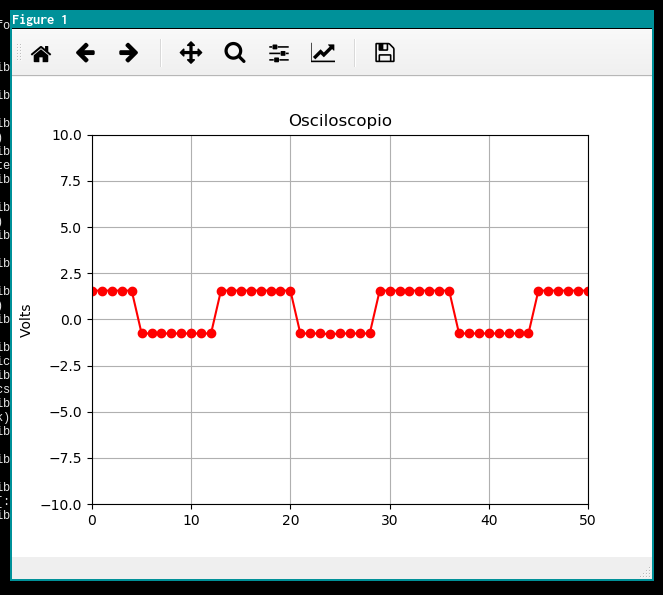
\includegraphics[scale=0.2]{Osc1.png}
\end{subfigure}
\begin{subfigure}{0.5\textwidth}
\centering
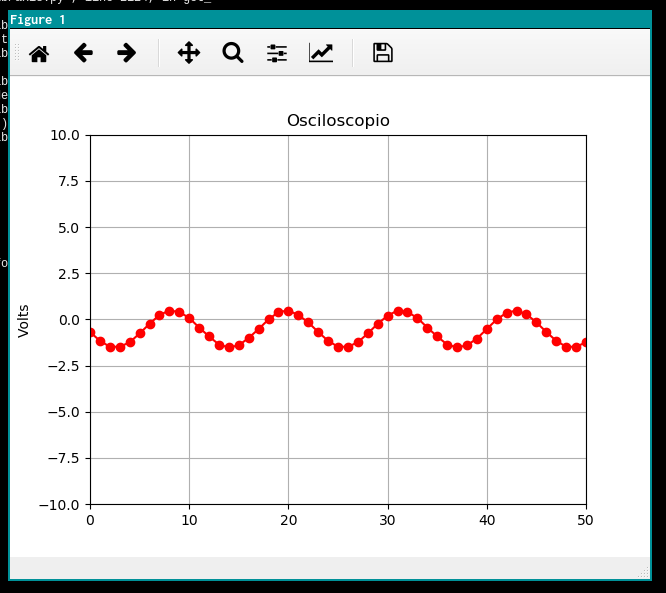
\includegraphics[scale=0.2]{Osc2.png}
\end{subfigure}
\caption{Resultados}
\label{Fig:Res}
\end{figure}

\section{Conclusión}
Este proyecto si bien es económico en comparación a conseguir un osciloscopio
“Profesional” cuenta con la gran desventaja de no ser tan exacto como el otro, aparte
carece de todas las funciones adicionales que posee el antes mencionado. Esto lleva a que
este proyecto sea un último recurso en caso de necesitarse un osciloscopio o bien hace que
quede como un proyecto “recreativo”.\\
La más grande dificultad encontrada durante la realización de este proyecto fue el poder
realizar gráficas en tiempo real de los datos que proporciona Arduino ya que si no se
podía graficar así realmente el proyecto no funcionaba. Se buscó en muchas páginas web
opciones, sin embargo, muy pocas realmente proporcionaban una forma de realizar dicha
acción.\\
El segundo mayor problema fue encontrar la manera de hacer que Arduino, de alguna manera,
pudiera “leer” voltaje negativo. Se intentó usar off set del generador de funciones  pero
esa alternativa era un tanto imprecisa y complicaba un poco la programación, por lo que se
buscó otra alternativa.\\
Como tercera dificultad se encontraba en valor máximo de voltaje que se debe proporcionar
a Arduino.\\
Estos últimos dos problemas se pudieron solucionar con un solo circuito, el cual, “mapea”
el voltaje que se le proporciona y lo manda a un rango de 0 - 5 volts.\\
Una manera de mejorar este proyecto es incorporarle funciones adicionales en la
programación para que, al desplegar en pantalla el voltaje, también pueda proporcionar
otros valores, ya sea RMS, frecuencia, etc., además de que pierde precisión conforme la
frecuencia de la onda de entrada aumenta debido a que Arduino no muestrea a intervalos
regulares, de nuevo esto puede ser solucionado con unos cambios en el programa de
Arduino, además la precisión podría mejorarse con un circuito que divida el voltaje de
entrada en intervalos de 0 a 5 volts dirigidos a distintos puertos analógicos para tener
mas puntos de muestreo.

\section{Referencias}
$$https://www.open-electronics.org/guest_projects/a-pc-and-an-arduino-heres-your-diy-oscilloscope/$$
$$http://www.instructables.com/id/Arduino-Oscilloscope-poor-mans-Oscilloscope/$$
$$https://www.build-electronic-circuits.com/arduino-oscilloscope/$$
\end{document}
